\section{Beispielreport}
    % \subsection{Mögliche Formate}
    %     \begin{frame}{\secname: \subsecname}
    %         \begin{itemize}
    %             \item Ausgabe ist möglich als reiner Text (auf der Konsole oder in einer Datei gespeichert),
    %             \item im Markdown-Format oder
    %             \item als HTML-Datei mit eigenem CSS und JavaScript
    %         \end{itemize}
    %     \end{frame}

    \subsection{Verwendete Software}
        \begin{frame}{\secname: \subsecname}
            \begin{itemize}
                \item Terminaldateimanager cfiles (Stand vom 17. Januar 2019)
                \item In C geschrieben
                \item Typische Sicherheitslücken
                \item Schwachstellen mittlerweile korrigiert
                \item Insgesamt mit vier Senken-Regeln 24 Verschmutzungen und 31 Senken gefunden
                \item Demo-Video
            \end{itemize}
        \end{frame}

    \subsection{Erkannte Verschmutzungen}
        \begin{frame}[fragile]{\secname: \subsecname}
            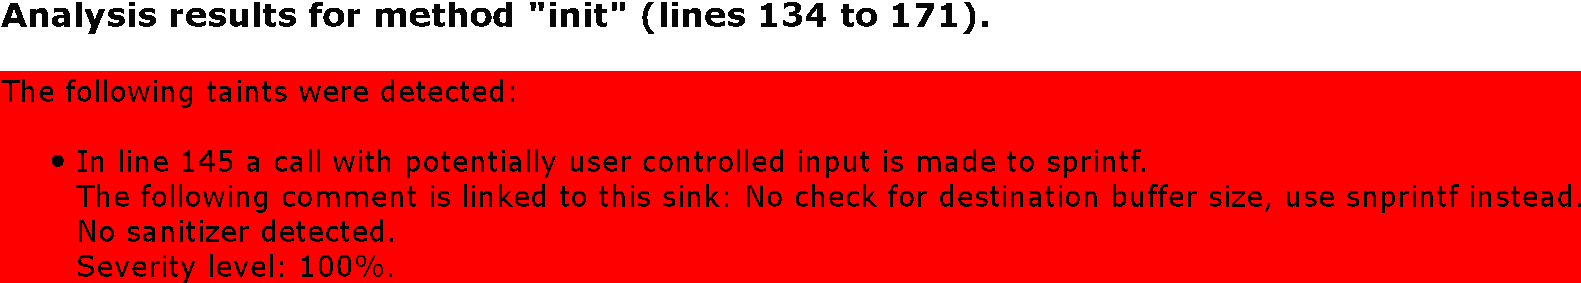
\includegraphics[keepaspectratio,height=\textheight,width=\columnwidth]{init-taint.pdf}
            \begin{lstlisting}[gobble=16, escapechar=!]
                char editor[20];
                void init()
                {
                    ...
                    // Set the editor
                    if( getenv("EDITOR") == NULL)
                        sprintf(editor, "%s", "vim");
                    else
                        !\colorbox{yellow}{sprintf(editor, "\%s", getenv("EDITOR"));}!
                    ...
                }
            \end{lstlisting}
        \end{frame}

    \subsection{Erkannte Senken}
        \begin{frame}[fragile]{\secname: \subsecname}
            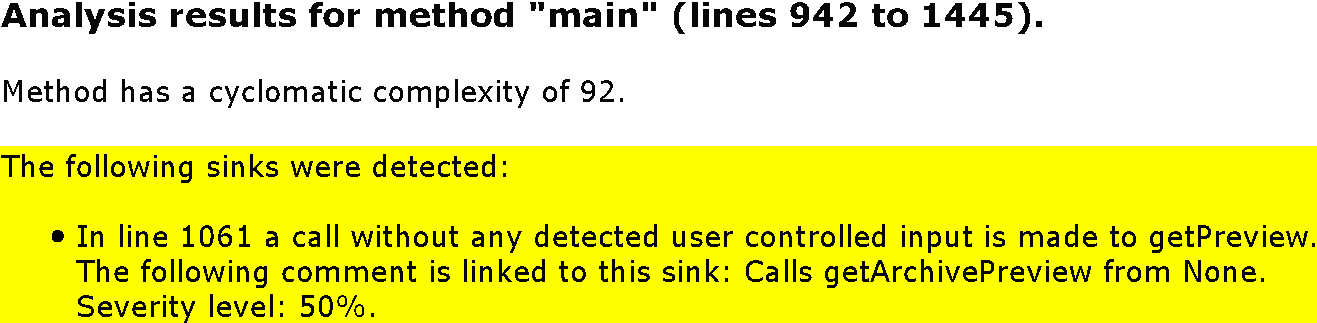
\includegraphics[keepaspectratio,height=\textheight,width=\columnwidth]{main-sink.pdf}
            \begin{lstlisting}[gobble=16, escapechar=!]
                int main(int argc, char* argv[]) {
                    ... !\colorbox{yellow}{getPreview(next\_dir,maxy,maxx/2+2);}! ...
                }
                void getPreview(char *filepath, int maxy, int maxx) {
                    ... !\colorbox{yellow}{getArchivePreview(filepath, maxy, maxx);}! ...
                }
                getArchivePreview(char *filepath, int maxy, int maxx) {
                    ... !\colorbox{yellow}{sprintf(temp\_dir,"atool -lq \textbackslash{}"\%s\textbackslash{}"\ > \textasciitilde/.cache/}!
                    !\colorbox{yellow}{cfiles/preview",filepath);}! ...
                }
            \end{lstlisting}
        \end{frame}
